% ============================================================
% FEE3411 Control Systems A -- Week 01, Part B, ABRIDGED
% Topic: Control system components and devices -- a conceptual survey
%
% This is a SECOND, shorter document covering only Part B of the Week 1
% notes. It carries the same figures and the same conclusions, but states
% the transfer functions as results instead of deriving them. The full
% derivations remain in Notes/week-01-notes.tex, which is unchanged and
% is still the reference document.
%
% Figures are copied verbatim from week-01-notes.tex. If a figure is
% corrected there, correct it here too -- they are not shared by \input.
%
% Build:  latexmk -pdf week-01-notes-partB-brief.tex
% Needs:  ../tex/preamble.tex (this file lives in Notes/).
% ============================================================
\documentclass[11pt,a4paper]{article}
\usepackage[margin=25mm]{geometry}
% ============================================================
% FEE3411 Control Systems A -- shared preamble
% Used by both the lecture notes (article) and the slides (beamer).
% ============================================================
\usepackage[T1]{fontenc}
% lmodern gives cleaner PDF fonts but is absent from minimal TeX installs.
% Load it only if present, so this preamble builds anywhere.
\IfFileExists{lmodern.sty}{\usepackage{lmodern}}{}
\usepackage{amsmath,amssymb,amsthm}
\usepackage{graphicx}
\usepackage{booktabs}
\usepackage{siunitx}
\usepackage{tikz}
\usepackage{circuitikz}
\usepackage{pgfplots}
\pgfplotsset{compat=1.18}
\usetikzlibrary{arrows.meta,positioning,calc,decorations.markings,shapes.geometric}
\usepackage[most]{tcolorbox}
\usepackage{xcolor}

% ---- Course colours -------------------------------------------------
\definecolor{fnavy}{HTML}{1F3864}
\definecolor{faccent}{HTML}{2E5E4E}
\definecolor{fflag}{HTML}{9C4221}

% ---- Block-diagram style --------------------------------------------
\tikzset{
  block/.style   = {draw, thick, rectangle, minimum height=2.6em,
                    minimum width=3.2em, align=center},
  sumnode/.style = {draw, thick, circle, inner sep=0pt, minimum size=1.6em},
  pickoff/.style = {fill, circle, inner sep=0pt, minimum size=3pt},
  sig/.style     = {-{Latex[length=2mm]}, thick},
}

% ---- Summing-junction signs -----------------------------------------
% \sumsign{<node>}{<angle>}{<+ or ->} places a sign just outside the circle.
\newcommand{\sumsign}[3]{\node[font=\small] at ($(#1)+(#2:0.5)$) {$#3$};}

% ---- Boxed environments ---------------------------------------------
\newtcolorbox{keyidea}[1][]{colback=fnavy!5,colframe=fnavy,
  fonttitle=\bfseries,title=Key idea,#1}
\newtcolorbox{workedex}[1][]{colback=faccent!5,colframe=faccent,
  fonttitle=\bfseries,title=Worked example,#1}
\newtcolorbox{pitfall}[1][]{colback=fflag!5,colframe=fflag,
  fonttitle=\bfseries,title=Common pitfall,#1}

% ---- Shorthands ------------------------------------------------------
\newcommand{\Lap}{\mathcal{L}}
\newcommand{\jw}{\mathrm{j}\omega}
\newcommand{\wn}{\omega_{n}}
\newcommand{\zt}{\zeta}
\newcommand{\TF}[1]{#1(s)}

% ---- Week title machinery -------------------------------------------
\usepackage{fancyhdr}
\newcommand{\thecoursecode}{FEE3411}
\newcommand{\thecoursename}{Control Systems A}
\newcommand{\wknum}{}
\newcommand{\wktopic}{}
\newcommand{\weeknumber}[1]{\renewcommand{\wknum}{#1}}
\newcommand{\weektopic}[1]{\renewcommand{\wktopic}{#1}}
\newcommand{\weektitle}{%
  \thispagestyle{plain}%
  \begin{center}
    {\large\sffamily\bfseries\color{fnavy}\thecoursecode: \thecoursename}\\[2pt]
    {\Huge\sffamily\bfseries Week \wknum}\\[4pt]
    {\LARGE\sffamily\color{fnavy}\wktopic}\\[6pt]
    \rule{\textwidth}{1.2pt}
  \end{center}\vspace{4pt}%
  \pagestyle{fancy}\fancyhf{}%
  \fancyhead[L]{\footnotesize\color{gray}\thecoursecode\ Week \wknum\ --- \wktopic}%
  \fancyhead[R]{\footnotesize\color{gray}\thepage}%
  \renewcommand{\headrulewidth}{0.4pt}%
}

% ---- Outcomes and reading boxes -------------------------------------
\newenvironment{outcomes}
  {\begin{tcolorbox}[colback=white,colframe=fnavy!60,
      fonttitle=\bfseries,title=By the end of this week you should be able to]
   \begin{itemize}[leftmargin=*]}
  {\end{itemize}\end{tcolorbox}}

\newtcolorbox{readingbox}{colback=gray!5,colframe=gray!50,
  fonttitle=\bfseries,title=Reading}

% enumitem must NOT be loaded under beamer: it overwrites beamer's itemize
% templates and the bullet markers silently disappear. The notes (article) get
% it; the slides (beamer) use beamer's own list machinery instead.
\makeatletter
\@ifclassloaded{beamer}{}{\usepackage{enumitem}}
\makeatother

\usepackage{float}  % [H] pins figures where they appear

% compact "where the maths lives" pointer -- a box per section was too bulky
\newcommand{\fullmath}[1]{%
  \par\smallskip\noindent
  \textcolor{fnavy}{\rule{\textwidth}{0.4pt}}\par\vspace{-4pt}
  {\small\textcolor{fnavy}{\textbf{Full treatment:}} \textit{#1}}\par\smallskip}

\weeknumber{1}
\weektopic{Part B --- Control System Components (Abridged)}

\begin{document}
\weektitle

\begin{center}
{\large\sffamily\bfseries\color{fnavy}A CONCEPTUAL SURVEY}
\end{center}

\bigskip
\begin{readingbox}
A shorter route through Part~B of the Week~1 notes: the same devices, the same
diagrams and the same conclusions, but the transfer functions are
\textbf{stated} rather than derived, and explained in words rather than algebra.
It does not replace \texttt{week-01-notes.pdf} --- each section carries a
\emph{Full treatment} line naming exactly where the derivation lives.

\smallskip
The syllabus outcome here is ELO~1, \emph{``describe the working principles''},
so describing is the requirement; the derivations belong to Week~2 and to
FEE3412. Nothing examinable in FEE3411 is lost by reading this version --- but
do not skim \S8, which is the idea the rest of the unit is built on.
\end{readingbox}

\bigskip
\begin{outcomes}
\item Say what each standard control component does, how it does it, and
      roughly what its transfer function looks like.
\item Choose sensibly between an electrical, hydraulic and pneumatic solution
      for a given job, and defend the choice.
\item Explain \emph{in words} why almost every positional actuator has the
      transfer function $K/[s(\tau s+1)]$, and why that single fact shapes
      Weeks 5, 6, 8 and 10.
\end{outcomes}

% ====================================================================
\section{Where the components sit}

Everything in this document is one of four boxes in a loop you have already
seen. Keep Figure~\ref{fig:chain} in view: when a later week labels a block
``actuator'', this is what is physically inside it.

\begin{figure}[H]
\centering
\resizebox{0.72\textwidth}{!}{%
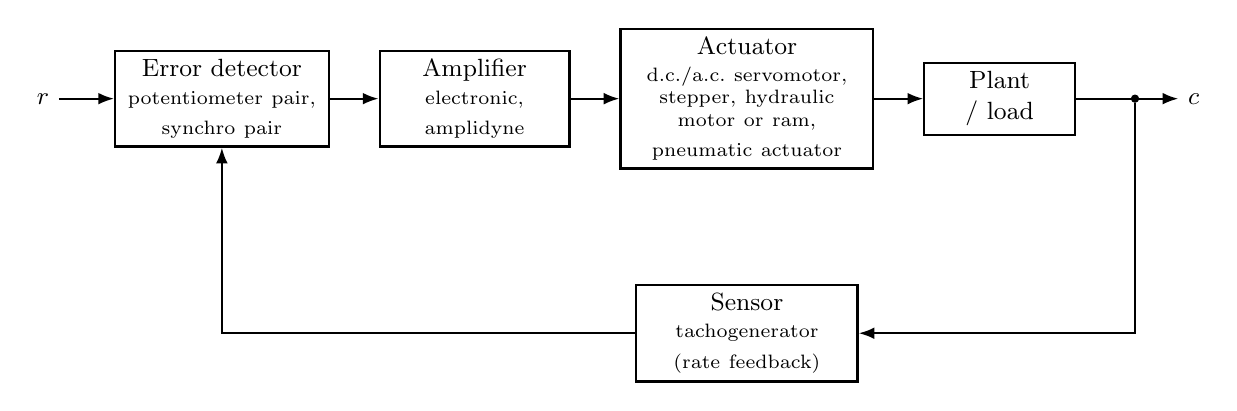
\begin{tikzpicture}[node distance=0.62cm, font=\small,
   bb/.style={block, align=center, inner sep=3pt}]
\node[bb, text width=2.5cm] (ed)
  {Error detector\\[2pt]{\scriptsize potentiometer pair,\\ synchro pair}};
\node[bb, right=of ed, text width=2.2cm] (am)
  {Amplifier\\[2pt]{\scriptsize electronic,\\ amplidyne}};
\node[bb, right=of am, text width=3.0cm] (ac)
  {Actuator\\[2pt]{\scriptsize d.c./a.c.\ servomotor,\\ stepper, hydraulic\\
   motor or ram,\\ pneumatic actuator}};
\node[bb, right=of ac, text width=1.7cm] (pl) {Plant\\/ load};
\node[bb, below=1.45cm of ac, text width=2.6cm] (se)
  {Sensor\\[2pt]{\scriptsize tachogenerator\\ (rate feedback)}};
\node[left=0.7cm of ed] (rr) {$r$};
\node[right=1.3cm of pl] (cc) {$c$};
\node[pickoff] at ($(pl.east)+(0.75,0)$) (po) {};
\draw[sig] (rr) -- (ed);
\draw[sig] (ed) -- (am);
\draw[sig] (am) -- (ac);
\draw[sig] (ac) -- (pl);
\draw[sig] (pl) -- (cc);
\draw[sig] (po) |- (se.east);
\draw[sig] (se) -| (ed);
\end{tikzpicture}}
\caption{Where each family of components sits in the loop. Everything in
Part~B is one of these four boxes.}
\label{fig:chain}
\end{figure}

\begin{keyidea}
There are only four jobs to do in a control loop: \textbf{measure the error},
\textbf{amplify it}, \textbf{act on the plant}, and \textbf{measure the
output}. Every device below is a way of doing one of those four things. When
you meet an unfamiliar component, the first question is which of the four it is.
\end{keyidea}

% ====================================================================
\section{Error detectors}

The error detector performs the subtraction $r-c$ \emph{physically}. Two
standard devices do it for angular position.

\subsection*{The potentiometer pair}

Two potentiometers share a d.c.\ supply; one is turned by the reference shaft,
the other by the load shaft. The voltage between the two wipers is proportional
to the difference between the shaft angles:
\[
  v_{e}=K_{p}\,(r-c),\qquad [K_{p}]=\si{\volt\per\radian}.
\]
The subtraction is done \emph{by the wiring}, not by a circuit. This is the
physical realisation of the summing junction you draw as $\otimes$.

\smallskip
\textbf{For:} cheap, d.c., and a \emph{pure gain} with no dynamics.
\textbf{Against:} the wiper is a sliding contact --- friction, wear, noise, and
a resolution set by the winding pitch.

\subsection*{The synchro pair}

Where the shaft turns continuously, through many revolutions, or sits in a
hostile environment, a sliding contact is unacceptable. The \textbf{synchro}
(trade names \emph{selsyn}, \emph{autosyn}) replaces it with transformer action
--- no contact anywhere in the signal path.

\begin{keyidea}
A synchro transmitter is a \textbf{transformer whose coupling depends on shaft
angle}. Its rotor coil is the primary; its three stator coils are the
secondaries; the voltage induced in each depends on the angle between that
coil and the rotor. Input a shaft angle, get out three a.c.\ voltages that
encode it.
\end{keyidea}

Wire those three stator leads to a second, similar machine --- a \textbf{control
transformer}, built with a cylindrical rotor so its output impedance does not
change as it turns --- and the flux pattern of the first is reproduced inside
the second. The voltage at the control transformer's rotor then depends on the
angle \emph{between the two rotors}. For small differences it is proportional
to that difference:
\[
  e(t)\;\approx\;K_{s}\,(\theta-\alpha)\,\sin\omega_{c}t,
  \qquad [K_{s}]=\si{\volt\per\radian}.
\]

\begin{figure}[H]
\centering
\resizebox{0.72\textwidth}{!}{%
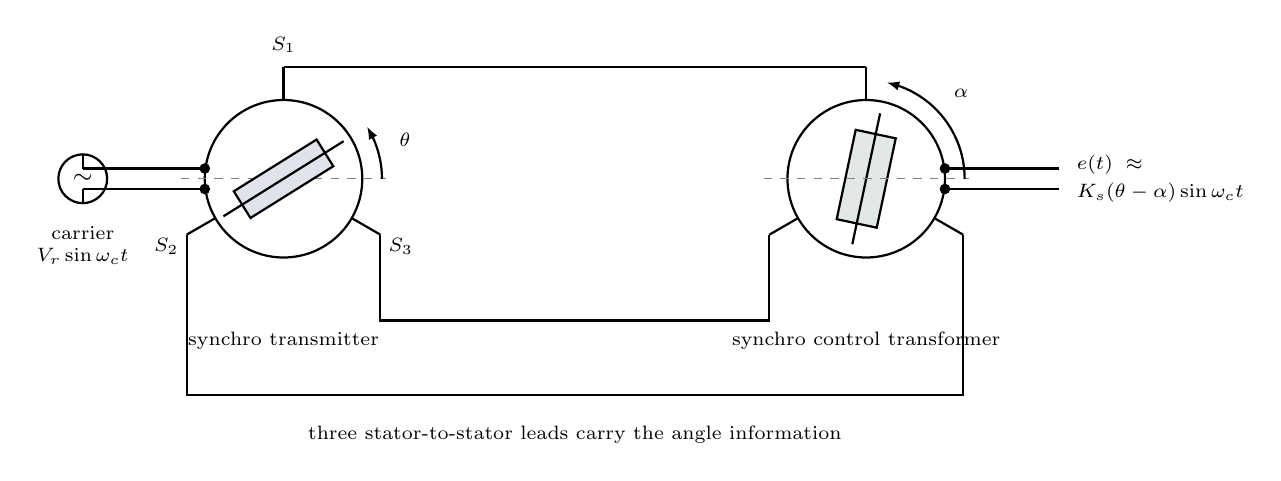
\begin{tikzpicture}[font=\small, x=1cm, y=1cm]
\def\R{1.0}\def\S{1.42}
% ================= transmitter =================
\draw[thick] (0,0) circle (\R);
\foreach \a in {90,210,330}{\draw[thick] (\a:\R) -- (\a:\S);}
\node[font=\scriptsize] at (90:{\S+0.28}) {$S_1$};
\node[font=\scriptsize] at (210:{\S+0.30}) {$S_2$};
\node[font=\scriptsize] at (330:{\S+0.30}) {$S_3$};
% rotor (single coil) at angle theta
\draw[dashed,gray] (-1.3,0) -- (1.3,0);
\begin{scope}[rotate=32]
  \draw[thick,fill=fnavy!14] (-0.62,-0.20) rectangle (0.62,0.20);
  \draw[thick] (-0.9,0) -- (0.9,0);
\end{scope}
\draw[thick,-{Latex[length=1.6mm]}] (1.25,0) arc (0:32:1.25);
\node[font=\scriptsize] at (18:1.62) {$\theta$};
\node[font=\scriptsize] at (0,-2.05) {synchro transmitter};
% slip rings and carrier supply (rotor leads out to the left)
\draw[fill] (-1.0,0.13) circle (1.7pt);
\draw[fill] (-1.0,-0.13) circle (1.7pt);
\draw[thick] (-1.0,0.13) -- (-2.55,0.13);
\draw[thick] (-1.0,-0.13) -- (-2.55,-0.13);
\draw[thick] (-2.55,0.13) -- (-2.55,0.30);
\draw[thick] (-2.55,-0.13) -- (-2.55,-0.30);
\draw[thick] (-2.55,0.30) circle (0) ;
\node[draw,thick,circle,minimum size=0.62cm] at (-2.55,0) {};
\node at (-2.55,0) {$\sim$};
\node[font=\scriptsize,align=center] at (-2.55,-0.85) {carrier\\$V_r\sin\omega_c t$};
% ================= control transformer =================
\begin{scope}[shift={(7.4,0)}]
\draw[thick] (0,0) circle (\R);
\foreach \a in {90,210,330}{\draw[thick] (\a:\R) -- (\a:\S);}
\begin{scope}[rotate=78]
  \draw[thick,fill=faccent!14] (-0.58,-0.26) rectangle (0.58,0.26);
  \draw[thick] (-0.85,0) -- (0.85,0);
\end{scope}
\draw[dashed,gray] (-1.3,0) -- (1.3,0);
\draw[thick,-{Latex[length=1.6mm]}] (1.25,0) arc (0:78:1.25);
\node[font=\scriptsize] at (42:1.62) {$\alpha$};
\node[font=\scriptsize] at (0,-2.05) {synchro control transformer};
% rotor output
\draw[fill] (1.0,0.13) circle (1.7pt);
\draw[fill] (1.0,-0.13) circle (1.7pt);
\draw[thick] (1.0,0.13) -- (2.45,0.13);
\draw[thick] (1.0,-0.13) -- (2.45,-0.13);
\node[font=\scriptsize,align=left,anchor=west] at (2.55,0)
   {$e(t)\;\approx$\\[2pt] $K_s(\theta-\alpha)\sin\omega_c t$};
\end{scope}
% ================= the three stator leads =================
\draw[thick] (0,\S) -- (7.4,\S);
\draw[thick] (-1.23,-0.71) -- (-1.23,-2.75) -- (8.63,-2.75) -- (8.63,-0.71);
\draw[thick] (1.23,-0.71) -- (1.23,-1.80) -- (6.17,-1.80) -- (6.17,-0.71);
\node[font=\scriptsize, align=center] at (3.7,-3.25)
   {three stator-to-stator leads carry the angle information};
\end{tikzpicture}}
\caption{Synchro transmitter and control transformer used as an error detector.
Cf.\ Nagrath \& Gopal Fig.~4.12, p.~94. The three
stator-to-stator leads carry the angle information; there is no sliding contact
in the signal path.}
\label{fig:synchro}
\end{figure}

The output is a carrier $\sin\omega_{c}t$ whose \emph{amplitude} carries the
error and whose \emph{phase flips} when the error changes sign. This is
\textbf{suppressed-carrier modulation}, and a loop whose internal signals look
like this is called a \textbf{carrier control system}.

\begin{pitfall}
In a carrier system the information is in the \textbf{envelope}, not the
instantaneous value. A student who reads the error straight off an oscilloscope
trace of $e(t)$, rather than its envelope, will conclude that the error is
oscillating at \SI{400}{\hertz} while the shaft is standing perfectly still.
\end{pitfall}

\fullmath{main notes \S5.2 (the coil voltages, the derivation of $e(t)$ from the rotor geometry, and where the small-angle approximation enters). Nagrath \& Gopal 2nd ed.\ \S4.3, p.~92.}

% ====================================================================
\section{Actuators}

\subsection*{The d.c.\ servomotor}

The workhorse --- a d.c.\ motor built for low inertia and rapid reversal.
\textbf{Armature control} (field constant, armature voltage varied) is used
almost universally; \textbf{field control} needs a cheaper amplifier but is
slower, because the field winding is highly inductive. Driving inertia and
friction, the armature-controlled motor has
\[
  \frac{\theta_{m}(s)}{V_{a}(s)}=\frac{K_{m}}{s(\tau_{m}s+1)} .
\]
Read that shape now and remember it --- \S8 is about why it keeps coming back.
In words: \emph{a constant voltage gives a constant speed} (hence the
integrator, since position is the accumulation of speed), \emph{and the motor
takes time to reach that speed} (hence the first-order lag, because inertia and
friction resist the change).

\smallskip
Large d.c.\ systems historically used an \textbf{amplidyne}, a rotating
cross-field power amplifier. Obsolete --- displaced by thyristor and IGBT
drives --- but the name appears in older textbook problems.

\subsection*{The a.c.\ (two-phase) servomotor}

Preferred at low power, and wherever a synchro error detector has already made
the signals a.c. Rugged, light, no brushes. Structurally it is a two-phase
induction motor: two stator windings \SI{90}{\degree} apart in space, excited
\SI{90}{\degree} apart in time, producing a rotating field that drags the rotor
round. Two design changes make it a servomotor:

\begin{enumerate}[leftmargin=*]
\item \textbf{High rotor resistance.} In an ordinary induction motor the
      reactance-to-resistance ratio is deliberately \emph{large}, which puts
      peak torque near the operating point --- and leaves part of the
      torque--speed curve \emph{positively} sloped.
\item \textbf{Unbalanced excitation.} One winding (the \emph{reference phase})
      is fed a fixed voltage; the other (the \emph{control phase}) is fed from
      the servo amplifier with a variable magnitude at
      $\pm\SI{90}{\degree}$. Reverse the sign of the control voltage and the
      motor reverses. The rotor is a small-diameter squirrel cage or a drag cup,
      to keep inertia low.
\end{enumerate}

\begin{figure}[H]
\centering
\resizebox{0.72\textwidth}{!}{%
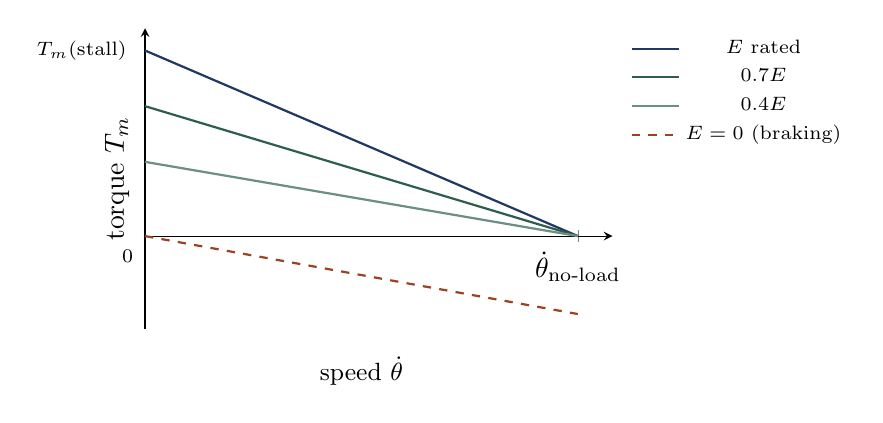
\begin{tikzpicture}
\begin{axis}[width=0.62\textwidth, height=5.4cm,
  ylabel={torque $T_m$},
  xmin=0, xmax=1.08, ymin=-0.5, ymax=1.12,
  xtick={0,1}, xticklabels={$0$,$\dot\theta_{\text{no-load}}$},
  ytick=\empty, axis y line=left, axis x line=middle, clip=false,
  legend style={font=\scriptsize, draw=none, at={(1.02,1.0)}, anchor=north west}]
\addplot[fnavy, thick, domain=0:1, samples=2]{1-x};
\addlegendentry{$E$ rated}
\addplot[faccent, thick, domain=0:1, samples=2]{0.7*(1-x)};
\addlegendentry{$0.7E$}
\addplot[faccent!70, thick, domain=0:1, samples=2]{0.4*(1-x)};
\addlegendentry{$0.4E$}
\addplot[fflag, thick, dashed, domain=0:1, samples=2]{-0.42*x};
\addlegendentry{$E=0$ (braking)}
\node[font=\scriptsize, anchor=east] at (axis cs:-0.02,1.0) {$T_m$(stall)};
\node[font=\scriptsize, anchor=north east] at (axis cs:-0.005,-0.02) {$0$};
\node[font=\small, anchor=north] at (axis cs:0.5,-0.60) {speed $\dot\theta$};
\end{axis}
\end{tikzpicture}}
\caption{Torque--speed characteristics of a two-phase servomotor at several
control-phase voltages, idealised as the straight lines used for linearisation.
All slopes are negative --- that is the whole point of the high-resistance
rotor. At zero control voltage the motor develops a \emph{decelerating} torque,
so that line passes through the origin with negative slope. Cf.\ Nagrath \&
Gopal Fig.~4.6, p.~86.}
\label{fig:acservo}
\end{figure}

\begin{keyidea}
Why the high rotor resistance matters is a \emph{stability} argument, and it is
worth following even without the algebra. The negative slope of the
torque--speed curve behaves exactly like extra viscous friction: the faster the
motor turns, the more the torque falls off, which damps it. A \emph{positive}
slope would behave like \emph{negative} friction --- negative damping --- and
the loop could oscillate on its own. That is why an ordinary induction motor
cannot be used as a servomotor, and it is your first sight of a theme that runs
to Week~12: stability considerations reach right down into the choice of
hardware.
\end{keyidea}

Its transfer function has the same shape as the d.c.\ motor's:
$\theta/E = K_{m}/[s(\tau_{m}s+1)]$.

\subsection*{The stepper motor}

A stepper converts a train of pulses into discrete angular steps ---
\textbf{one step per pulse}. It is the actuator of incremental motion control:
printers, tape and capstan drives, machine tools, plotters, 3-D printers.

In a \emph{variable-reluctance} stepper the toothed stator stacks are
pulse-excited and the toothed rotors are unexcited. Energise a stack and the
rotor is pulled to the nearest \textbf{minimum-reluctance} position, where the
teeth line up. Successive stator stacks are offset by
\[
  \alpha=\frac{360^{\circ}}{n\,T},
  \qquad n=\text{stacks (= phases)},\quad T=\text{rotor teeth},
\]
and that offset $\alpha$ is the \textbf{step angle}. Exciting the phases in the
order $abcabc\ldots$ steps the rotor one way, $bacbac\ldots$ the other ---
which is why \emph{directional control needs three or more phases}.

\begin{figure}[H]
\centering
\resizebox{0.72\textwidth}{!}{%
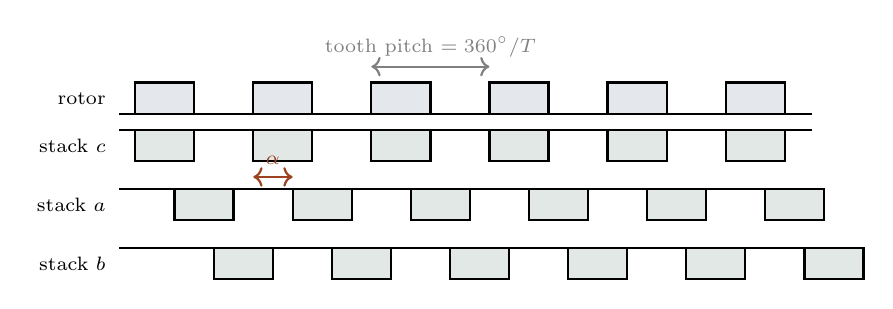
\begin{tikzpicture}[font=\small, scale=1.0]
% rotor teeth (aligned across all stacks)
\foreach \i in {0,...,5}{
  \draw[thick,fill=fnavy!12] ({\i*1.5},2.35) rectangle ({\i*1.5+0.75},2.75);}
\draw[thick] (-0.2,2.35) -- (8.6,2.35);
\node[left, font=\scriptsize] at (-0.25,2.55) {rotor};
% stack c : aligned
\foreach \i in {0,...,5}{
  \draw[thick,fill=faccent!14] ({\i*1.5},1.75) rectangle ({\i*1.5+0.75},2.15);}
\draw[thick] (-0.2,2.15) -- (8.6,2.15);
\node[left, font=\scriptsize] at (-0.25,1.95) {stack $c$};
% stack a : offset by alpha
\foreach \i in {0,...,5}{
  \draw[thick,fill=faccent!14] ({\i*1.5+0.5},1.0) rectangle ({\i*1.5+1.25},1.4);}
\draw[thick] (-0.2,1.4) -- (8.6,1.4);
\node[left, font=\scriptsize] at (-0.25,1.2) {stack $a$};
% stack b : offset by 2 alpha
\foreach \i in {0,...,5}{
  \draw[thick,fill=faccent!14] ({\i*1.5+1.0},0.25) rectangle ({\i*1.5+1.75},0.65);}
\draw[thick] (-0.2,0.65) -- (8.6,0.65);
\node[left, font=\scriptsize] at (-0.25,0.45) {stack $b$};
% dimension for alpha
\draw[<->, thick, fflag] (1.5,1.55) -- (2.0,1.55);
\node[fflag, font=\scriptsize, above] at (1.75,1.58) {$\alpha$};
% tooth pitch
\draw[<->, thick, gray] (3.0,2.95) -- (4.5,2.95);
\node[gray, font=\scriptsize, above] at (3.75,2.95) {tooth pitch $=360^\circ/T$};
\end{tikzpicture}}
\caption{Developed (rolled-out) view of a three-stack variable-reluctance
stepper. Rotor teeth are aligned across all stacks; stator stacks are offset
successively by $\alpha=360^\circ/nT$. Energising $c$, then $a$, then $b$ pulls
the rotor one step $\alpha$ at a time. Cf.\ Nagrath \& Gopal Figs.~4.18 and
4.20, pp.~100--101.}
\label{fig:stepper}
\end{figure}

\begin{keyidea}
The stepper is a \textbf{digital actuator}: shaft position is determined
entirely by the pulse count. An \emph{open-loop} step servo can therefore reach
the accuracy of a closed-loop analogue system with no position sensor at all
--- the rare case where open loop is the right engineering answer.
\end{keyidea}

\begin{pitfall}
The price is \textbf{skipped steps}. If pulses arrive faster than the rotor can
settle, or the rotor oscillates too much about the lock position, a step is
lost --- and since nothing is measured, it is lost \emph{silently and
permanently}. High-performance systems close the loop after all, gating the
pulse train from a position feedback signal.
\end{pitfall}

Stepper dynamics are genuinely nonlinear and are solved numerically --- one
reason steppers do not reappear in the analysis weeks.

\fullmath{main notes \S6 (the Taylor-series linearisation of the a.c.\ servomotor's torque--speed surface, the stall-torque and no-load-speed tests that give $K$ and $f$, and the reluctance-torque model of the stepper). Nagrath \S4.3, p.~84 (a.c.\ servomotor) and \S4.4, p.~99 (stepper).}

% ====================================================================
\section{Sensors: the tachogenerator}

A \textbf{tachogenerator} produces a voltage proportional to shaft speed:
\[
  v_{t}=K_{t}\,\dot\theta,\qquad
  [K_{t}]=\si{\volt\per\radian\per\second}.
\]
A \emph{d.c.} tachogenerator is a small permanent-magnet generator (commutation
ripple is its main limitation); an \emph{a.c.\ drag-cup} type uses a thin
aluminium cup as its rotor, for very low inertia.

It is used two ways: as the \textbf{sensor of a speed loop}, where speed is the
controlled variable; and as \textbf{rate feedback} inside a \emph{position}
loop, where the speed signal is subtracted in an inner loop purely to add
damping.

\begin{keyidea}
The second use is the interesting one. Adding rate feedback changes
\emph{only} the damping of the closed-loop system; it leaves the steady-state
gain alone. So you can calm an oscillatory servo without making it less
accurate.

That is your first sight of a \textbf{compensator} --- a component added not
because the plant needs it to function, but because the \emph{loop} needs it to
behave. We use it as a design tool in Week~9; FEE3412 studies it properly.
\end{keyidea}

\fullmath{main notes \S7, which works through Nagrath's a.c.\ position control system and shows the tachometer constant $K_{t}$ appearing only in the $s$ coefficient of the closed-loop denominator, i.e.\ only in the damping term. Nagrath \S4.3, p.~88 (tachometer) and p.~96 (the full system).}

% ====================================================================
\section{Hydraulic power elements}

Where the load is large, hydraulics win: a hydraulic motor is far smaller than
an electric one of the same power, and the components are fast and very stiff
under load. Against that --- leaks, sealing, noise, sluggishness when cold, and
inflexible lines. Typical uses: power steering and brakes, ship steering gear,
machine tools, aircraft flight controls, excavators.

Output devices split by motion: \textbf{rotary} --- \emph{hydraulic motors},
which is what the syllabus calls ``rotary actuators''; and
\textbf{translational} --- \emph{linear actuators}, i.e.\ cylinders and rams.

\subsection*{Pump--motor transmission}

A \textbf{variable-stroke pump} driving a \textbf{fixed-stroke motor}, both
axial-piston machines whose pistons bear on a wobble plate. Tilt the plate
through the \emph{stroke angle} and oil is delivered in proportion to the tilt;
reverse the tilt and the motor reverses. One mechanical variable controls
everything. A flow balance and a torque balance give
$\theta/X = K/[s(\tau s+1)]$ --- the same shape as the electric motors.

\subsection*{Valve control, and the cylinder}

Instead of varying the pump stroke, hold the supply pressure constant and
throttle the flow with a \textbf{spool valve}. Its moving part is far lighter
than a pump's stroke mechanism, so time constants shrink and the system becomes
much faster. The cost: valve flow is nonlinear --- through a sharp-edged orifice
it goes as $\sqrt{\Delta p}$ --- so the model we use is a \emph{linearisation},
valid only for small movements about neutral.

\begin{figure}[H]
\centering
\resizebox{0.72\textwidth}{!}{%
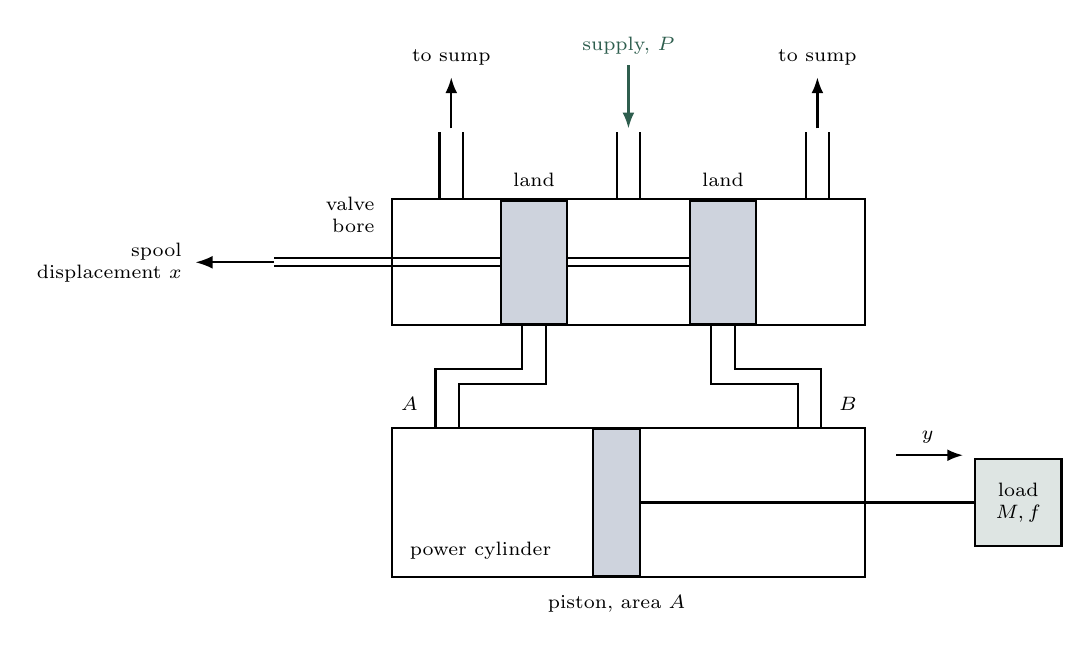
\begin{tikzpicture}[font=\small, x=1cm, y=1cm]
% ---------------- valve body (bore) ----------------
\draw[thick] (0.6,4.6) rectangle (6.6,6.2);
\node[font=\scriptsize, left, align=right] at (0.5,6.0) {valve\\bore};
% ---------------- spool: stem + two lands ----------------
\draw[thick] (-0.9,5.35) -- (2.4,5.35);
\draw[thick] (-0.9,5.45) -- (2.4,5.45);
\draw[thick] (2.4,5.35) -- (4.8,5.35);
\draw[thick] (2.4,5.45) -- (4.8,5.45);
\foreach \c in {2.4,4.8}{
  \draw[thick,fill=fnavy!22] (\c-0.42,4.62) rectangle (\c+0.42,6.18);}
\node[font=\scriptsize, above] at (2.4,6.24) {land};
\node[font=\scriptsize, above] at (4.8,6.24) {land};
\draw[thick,-{Latex[length=2.2mm]}] (-0.9,5.4) -- (-1.9,5.4);
\node[font=\scriptsize, left, align=right] at (-1.95,5.4)
      {spool\\displacement $x$};
% ---------------- ports on the top face ----------------
% supply, centre
\draw[thick] (3.45,6.2) -- (3.45,7.05);
\draw[thick] (3.75,6.2) -- (3.75,7.05);
\draw[sig, faccent] (3.6,7.9) -- (3.6,7.1);
\node[faccent, font=\scriptsize, above, align=center] at (3.6,7.92)
      {supply, $P$};
% two sump returns, outer
\foreach \c in {1.35,6.0}{
  \draw[thick] (\c-0.15,6.2) -- (\c-0.15,7.05);
  \draw[thick] (\c+0.15,6.2) -- (\c+0.15,7.05);
  \draw[sig] (\c,7.1) -- (\c,7.75);
  \node[font=\scriptsize, above] at (\c,7.78) {to sump};}
% ---------------- service ports on the bottom face ----------------
\draw[thick] (2.25,4.6) -- (2.25,4.05) -- (1.15,4.05) -- (1.15,3.3);
\draw[thick] (2.55,4.6) -- (2.55,3.85) -- (1.45,3.85) -- (1.45,3.3);
\node[font=\scriptsize, left] at (1.05,3.6) {$A$};
\draw[thick] (4.65,4.6) -- (4.65,3.85) -- (5.75,3.85) -- (5.75,3.3);
\draw[thick] (4.95,4.6) -- (4.95,4.05) -- (6.05,4.05) -- (6.05,3.3);
\node[font=\scriptsize, right] at (6.15,3.6) {$B$};
% ---------------- power cylinder ----------------
\draw[thick] (0.6,1.4) rectangle (6.6,3.3);
\draw[thick,fill=fnavy!22] (3.15,1.42) rectangle (3.75,3.28);
\node[font=\scriptsize, below] at (3.45,1.3) {piston, area $A$};
\node[font=\scriptsize, above right] at (0.7,1.5) {power cylinder};
% rod and load
\draw[very thick] (3.75,2.35) -- (8.0,2.35);
\draw[thick,fill=faccent!16] (8.0,1.8) rectangle (9.1,2.9);
\node[font=\scriptsize, align=center] at (8.55,2.35) {load\\$M,f$};
\draw[sig] (7.0,2.95) -- (7.85,2.95);
\node[font=\scriptsize, above] at (7.4,2.98) {$y$};
\end{tikzpicture}}
\caption{Four-way spool valve controlling a double-acting power cylinder --- a
hydraulic linear actuator. Spool displacement $x$ admits high-pressure oil to
one side of the piston and vents the other to sump; the differential pressure
drives the load a distance $y$. Cf.\ Nagrath \& Gopal Fig.~4.27, p.~111
(the section begins on p.~110).}
\label{fig:spool}
\end{figure}

The cylinder's transfer function is, again, $Y/X = K/[s(\tau s+1)]$.

\begin{pitfall}
\textbf{Where the $1/s$ comes from --- this is the important sentence in the
whole document.} It is not an approximation and it is not inertia. Flow into a
cylinder sets the piston's \emph{velocity}; position is therefore the
accumulation of that velocity. \textbf{Any actuator whose input commands a
rate} --- valve opening $\to$ velocity, armature voltage $\to$ speed, pump
stroke $\to$ motor speed --- carries a free integrator when the output you care
about is position.
\end{pitfall}

\fullmath{main notes \S8 (the continuity and torque balances, the leakage and compressibility flow terms, and the linearised valve relation $q=K_{1}x-K_{2}p$). Nagrath \S4.5: pumps and motors p.~104, valves p.~108, linear actuator p.~110.}

% ====================================================================
\section{Pneumatic power elements}

Air instead of oil: non-inflammable, intrinsically safe, and with a viscosity
that is negligible and stable with temperature. But air is
\textbf{compressible}, so pneumatic systems carry substantial compressibility
flow and are characterised by \textbf{longer time delays} --- which is why they
dominate in \emph{process} control, where the plant is slow anyway, and are rare
where speed matters.

\begin{description}[leftmargin=*, style=nextline]
\item[Bellows] A thin corrugated chamber that behaves as a spring: pressure in,
  displacement out, with no dynamics --- a \emph{pure gain} $A/K$.
\item[Flapper--nozzle valve] The key sensing element. Air at constant supply
  pressure passes through a fixed orifice and out of a nozzle; a pivoted flapper
  sits close to the nozzle. Move the flapper nearer and the restriction rises,
  so the back pressure climbs towards the supply; move it away and the pressure
  falls towards ambient. A very small movement produces a very large pressure
  change --- a high-gain displacement-to-pressure transducer.
\item[Pneumatic relay] Keeping the flapper movement small enough to stay linear
  also keeps the output pressure swing small, so a pneumatic \emph{power
  amplifier} is added in cascade. A ball seats to either connect the output to
  supply or vent it to atmosphere. The relay also inverts the sign.
\item[Diaphragm actuator] Provides the translational output most pneumatic
  systems need: pressure acts on a diaphragm, which drives a stem against a
  return spring.
\end{description}

\begin{figure}[H]
\centering
\resizebox{0.72\textwidth}{!}{%
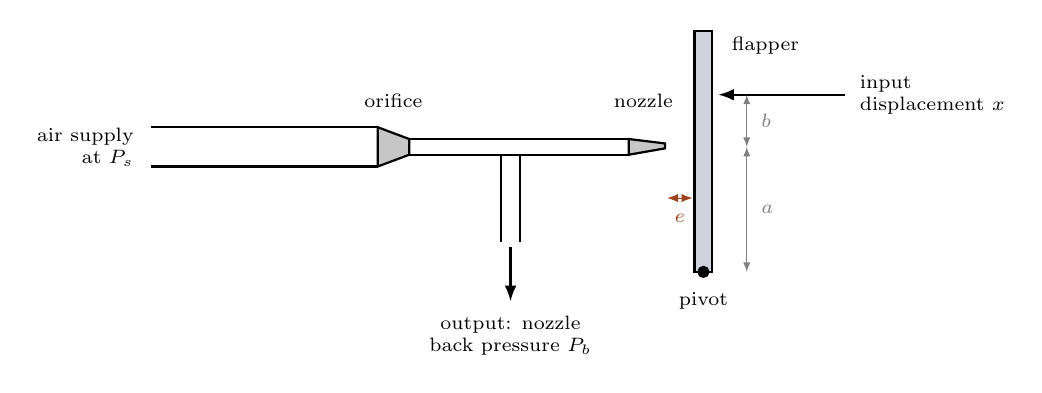
\begin{tikzpicture}[font=\small, x=1.25cm, y=1.25cm]
% ---- supply line and fixed orifice ----
\draw[thick] (0,1.62) -- (2.3,1.62);
\draw[thick] (0,2.02) -- (2.3,2.02);
\node[font=\scriptsize, left, align=right] at (-0.08,1.82)
      {air supply\\at $P_s$};
\draw[thick,fill=gray!45] (2.3,2.02) -- (2.62,1.90) -- (2.62,1.74)
                          -- (2.3,1.62) -- cycle;
\node[font=\scriptsize, above] at (2.46,2.12) {orifice};
% ---- chamber up to the nozzle ----
\draw[thick] (2.62,1.90) -- (4.85,1.90);
\draw[thick] (2.62,1.74) -- (4.85,1.74);
% ---- back-pressure tap ----
\draw[thick] (3.55,1.74) -- (3.55,0.85);
\draw[thick] (3.75,1.74) -- (3.75,0.85);
\draw[sig] (3.65,0.80) -- (3.65,0.25);
\node[font=\scriptsize, below, align=center] at (3.65,0.20)
      {output: nozzle\\back pressure $P_b$};
% ---- nozzle ----
\draw[thick,fill=gray!45] (4.85,1.90) -- (5.22,1.855) -- (5.22,1.805)
                          -- (4.85,1.74) -- cycle;
\node[font=\scriptsize, above] at (5.0,2.12) {nozzle};
% ---- flapper on a pivot ----
\draw[thick,fill=fnavy!22] (5.52,0.55) rectangle (5.70,3.00);
\node[font=\scriptsize, right] at (5.80,2.85) {flapper};
\draw[fill] (5.61,0.55) circle (2pt);
\node[font=\scriptsize, below] at (5.61,0.44) {pivot};
% ---- the gap e ----
\draw[{Latex[length=1.4mm]}-{Latex[length=1.4mm]}, fflag]
      (5.24,1.30) -- (5.50,1.30);
\node[fflag, font=\scriptsize, below] at (5.37,1.24) {$e$};
% ---- input displacement ----
\draw[sig] (7.05,2.35) -- (5.76,2.35);
\node[font=\scriptsize, right, align=left] at (7.10,2.35)
      {input\\displacement $x$};
% ---- lever arms ----
\draw[{Latex[length=1.2mm]}-{Latex[length=1.2mm]}, gray]
      (6.05,0.55) -- (6.05,1.82);
\node[gray, font=\scriptsize, right] at (6.10,1.19) {$a$};
\draw[{Latex[length=1.2mm]}-{Latex[length=1.2mm]}, gray]
      (6.05,1.82) -- (6.05,2.35);
\node[gray, font=\scriptsize, right] at (6.10,2.09) {$b$};
\end{tikzpicture}}
\caption{Flapper--nozzle valve. Small movements of the flapper produce large
changes in back pressure --- a high-gain displacement-to-pressure transducer.
Cf.\ Nagrath \& Gopal Fig.~4.34, p.~117.}
\label{fig:flapper}
\end{figure}

\begin{figure}[H]
\centering
\resizebox{0.72\textwidth}{!}{%
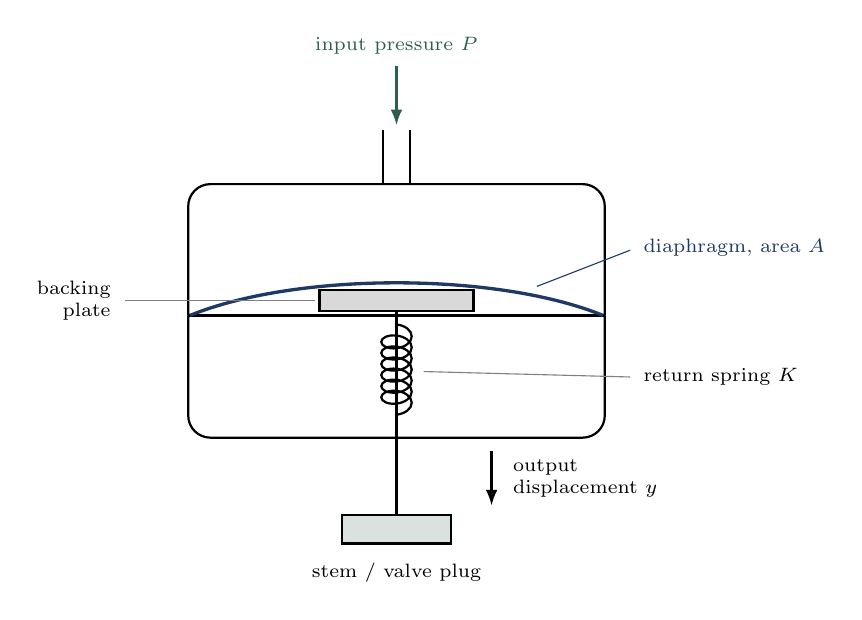
\begin{tikzpicture}[font=\small, x=1.15cm, y=1.15cm]
% ---- housing ----
\draw[thick, rounded corners=8pt] (0.7,2.30) -- (0.7,3.75) -- (5.3,3.75)
                                  -- (5.3,2.30);
\draw[thick, rounded corners=8pt] (0.7,2.30) -- (0.7,0.95) -- (5.3,0.95)
                                  -- (5.3,2.30);
\draw[thick] (0.7,2.30) -- (5.3,2.30);
% ---- diaphragm ----
\draw[very thick, fnavy] (0.72,2.30) .. controls (1.9,2.78) and (4.1,2.78)
                         .. (5.28,2.30);
\node[fnavy, font=\scriptsize, anchor=west] at (5.62,3.05)
     {diaphragm, area $A$};
\draw[fnavy] (5.58,3.02) -- (4.55,2.62);
% ---- pressure inlet ----
\draw[thick] (2.85,3.75) -- (2.85,4.35);
\draw[thick] (3.15,3.75) -- (3.15,4.35);
\draw[sig, faccent] (3.0,5.05) -- (3.0,4.40);
\node[faccent, font=\scriptsize, above] at (3.0,5.08) {input pressure $P$};
% ---- backing plate ----
\draw[thick,fill=gray!30] (2.15,2.35) rectangle (3.85,2.58);
\node[font=\scriptsize, anchor=east, align=right] at (-0.05,2.46)
     {backing\\plate};
\draw[gray] (0.0,2.46) -- (2.10,2.46);
% ---- stem ----
\draw[very thick] (3.0,2.35) -- (3.0,0.10);
% ---- return spring ----
\draw[thick, decorate, decoration={coil, aspect=0.6, segment length=4pt,
      amplitude=5.5pt}] (3.0,2.20) -- (3.0,1.15);
\node[font=\scriptsize, anchor=west] at (5.62,1.62) {return spring $K$};
\draw[gray] (5.58,1.62) -- (3.30,1.68);
% ---- output ----
\draw[sig] (4.05,0.80) -- (4.05,0.20);
\node[font=\scriptsize, anchor=west, align=left] at (4.18,0.50)
     {output\\displacement $y$};
\draw[thick,fill=faccent!18] (2.40,-0.22) rectangle (3.60,0.10);
\node[font=\scriptsize, below] at (3.0,-0.33) {stem / valve plug};
\end{tikzpicture}}
\caption{Pneumatic diaphragm actuator. Unlike the hydraulic cylinder, the spring
gives it a definite equilibrium position for each pressure --- so its transfer
function is second order with \emph{no} free integrator.
Cf.\ Nagrath \& Gopal Fig.~4.37, p.~119.}
\label{fig:pneuact}
\end{figure}

\begin{pitfall}
Compare the two actuators. The hydraulic cylinder has a free $1/s$; the
spring-loaded pneumatic diaphragm does \textbf{not} --- it is
$A/(Ms^{2}+fs+K)$, an ordinary second-order lag.

The difference is the \textbf{spring}. With a spring, a constant pressure gives
a constant \emph{position}, because the spring force balances the applied force
at a definite displacement. Without one, a constant flow gives a constant
\emph{velocity}. Read the physics, not the picture.
\end{pitfall}

\fullmath{main notes \S9 (the force balances giving each transfer function, and the lever-arm factor $a/(a+b)$ in the flapper gain). Nagrath \S4.6: bellows p.~116, flapper valve p.~117, relay p.~118, actuator p.~119.}

% ====================================================================
\section{Choosing between them}

\begin{center}
\begin{tabular}{@{}p{0.185\textwidth}p{0.245\textwidth}p{0.245\textwidth}p{0.245\textwidth}@{}}
\toprule
 & \textbf{Electric} & \textbf{Hydraulic} & \textbf{Pneumatic}\\
\midrule
Working medium & electric current & incompressible oil & compressible air\\
Power/weight & moderate & very high & low\\
Speed of response & fast & fastest under load & slow (compressibility)\\
Stiffness under load & moderate & very high & low\\
Typical use & instruments, servos, drives & machine tools, steering, aircraft
controls, presses & process control valves\\
Main drawback & limited torque density & leaks, sealing, contamination, noise &
long time delays, low stiffness\\
Safety & sparks & fire risk from oil mist & non-inflammable, intrinsically
safe\\
\bottomrule
\end{tabular}
\end{center}

\begin{keyidea}
The table is not a list to memorise; it is three trade-offs to reason with.
\textbf{Power density} pushes you towards hydraulics, \textbf{safety and cost}
towards pneumatics, \textbf{precision and convenience} towards electrics. Almost
every real selection is one of those three arguments winning.
\end{keyidea}

% ====================================================================
\section{One shape, over and over}

Collect what the survey produced. Note that the \emph{physics} of these devices
have almost nothing in common --- current and flux, oil under pressure,
compressed air --- and yet:

\begin{center}
\begin{tabular}{@{}p{0.27\textwidth}cp{0.42\textwidth}@{}}
\toprule
\textbf{Device} & \textbf{Shape} & \textbf{Why}\\
\midrule
d.c.\ servomotor & $\dfrac{K}{s(\tau s+1)}$
  & voltage commands \emph{speed}; inertia and friction resist\\[6pt]
a.c.\ servomotor & $\dfrac{K}{s(\tau s+1)}$
  & control voltage commands \emph{speed}; same resistance\\[6pt]
Hydraulic transmission & $\dfrac{K}{s(\tau s+1)}$
  & stroke angle commands \emph{motor speed}\\[6pt]
Hydraulic cylinder & $\dfrac{K}{s(\tau s+1)}$
  & valve opening commands \emph{piston velocity}\\
\addlinespace
Potentiometer, synchro, tachogenerator, bellows
  & pure gain & they \emph{report} a quantity; nothing accumulates\\
\addlinespace
Pneumatic diaphragm actuator & $\dfrac{A}{Ms^{2}+fs+K}$
  & the spring fixes a \emph{position} for each pressure, so nothing
    accumulates\\
\bottomrule
\end{tabular}
\end{center}

\begin{keyidea}
Almost every \textbf{positional actuator} in control engineering, whatever its
physics, has the transfer function
\[
  G(s)=\frac{K}{s(\tau s+1)} .
\]
The $\mathbf{1/s}$ is there because \textbf{the input commands a rate} and the
output of interest is the accumulation of that rate. The
$\mathbf{1/(\tau s+1)}$ is there because \textbf{inertia and friction resist}
that rate. Sensors and error detectors, by contrast, are usually
\textbf{pure gains} --- they report, they do not accumulate.

The exception proves the rule: put a spring on the output and the accumulation
stops, and with it the integrator.
\end{keyidea}

This is not a curiosity to note and forget. It is the reason a single body of
mathematics carries the whole unit, and it is why the weeks ahead look the way
they do:

\begin{itemize}[leftmargin=*]
\item Put $K/[s(\tau s+1)]$ in a unity-feedback loop and you get a
      \textbf{second-order system} --- \emph{Week 5}, and its $\zt$ and $\wn$.
\item The free integrator makes the open loop \textbf{type 1}: it tracks a step
      with zero steady-state error, a ramp with a finite one --- \emph{Week 6}.
\item Its pole--zero pattern --- one pole at the origin, one on the negative
      real axis --- gives the most common \textbf{root locus} you will ever
      sketch --- \emph{Week 8}.
\item Its \textbf{Bode plot} is a $-\SI{20}{\decibel}$/decade line plus a single
      corner --- \emph{Week 10}.
\end{itemize}

\begin{keyidea}
If you take one thing from Part~B, take this: \textbf{you have already met the
plant you will study for the next eleven weeks.} The hardware survey was not a
digression before the real course --- it was the course, in physical form.
\end{keyidea}

% ====================================================================
\section*{Where the mathematics lives}

Everything stated here without proof is derived in \texttt{week-01-notes.pdf} ---
the \emph{Full treatment} line under each section above names the exact place.

\smallskip\noindent
The primary hardware source throughout is \textbf{Nagrath \& Gopal, 2nd
edition, Chapter 4} (pp.~84--121), with the potentiometer servomechanism at
\S5.4, p.~137. Beware: Nagrath's section numbering is \emph{not} stable across
editions, so check any page number against the copy you actually hold.

\section*{Looking ahead}

Part~A gave you the vocabulary; this document gave you the hardware. From
Week~2 the subject becomes mathematical, and it does so by taking exactly these
devices and deriving from first principles the transfer functions quoted here
without proof --- starting with the armature-controlled d.c.\ servomotor
driving a load through a gear train.

Two boundaries worth restating. \emph{Components are survey depth in FEE3411}:
you need to describe working principles, not design a servomotor or select a
valve. And \emph{FEE3411 owns analysis while FEE3412 owns design} --- FEE3412
contains a full hardware block and will treat all of this properly.

\end{document}
